\chapter{Architektura rozwiązania}
\section{Architektura aplikacji}
Struktura aplikacji jest oparta na podziale narzuconym przez wykorzystany framework Django. Zgodnie z tym założeniem projekt dzieli się na poszczególne moduły, które nazywane są paczkami.  W aplikacji można wyróżnić cztery podstawowe elementy kolejno odpowiadające za zarządzanie eksperymentami i użytkownikami, graficzny interfejs użytkownika oraz moduł, który scala te elementy w całość. Schemat modułów jest przedstawiony na Rys. \ref{rys4_packages}. 

Aplikacja została zaimplementowana zgodnie ze stylem architektonicznym REST (\textit{Representational State Transfer}). Do komunikacji pomiędzy widokami aplikacji, a logiką biznesową znajdującą się na serwerze, wykorzystywany będzie protokół http. W tym celu do każdej poszczególnej funkcjonalności działającej w projekcie musiał zostać wystawiony punkt końcowy. Taki rodzaj rozwiązania zapewnia jasny podział na poszczególne warstwy, które są od siebie niezależne. Dzięki temu część serwerowa aplikacji może działać nie ingerując w część interfejsu graficznego. Mapowaniem poszczególnych modułów aplikacji na punkty końcowe zajmuje się główny moduł \enquote{decisionTree}. 


Dane użytkowników będą przetrzymywane w katalogu \enquote{users} i odpowiednim podkatalogu o nazwie loginu danego użytkownika. Każdy użytkownik może wgrywać dowolną ilość plików z danymi (o rozszerzeniach \enquote{*.xml}, \enquote{*.data}, \enquote{*.test} oraz \enquote{*.names} do swojego folderu). Podczas tworzenia nowego eksperymentu tworzony jest dla niego katalog o nazwie składającej się z pola  \enquote{id} i \enquote{name}. Tam są przechowywane wszystkie pliki  związane z zadaniem. Użytkownik będzie miał możliwość pobrania całego folderu z plikami eksperymentu w postaci archiwum o rozszerzeniu  \enquote{*.zip}. Dodatkowy wariant w aplikacji pozwali na zarządzanie katalogiem głównym użytkownika. Udostępnione są opcje do zmiany nazwy, usunięcia czy też pobrania pliku. 

\begin{figure}[htb]
	\centering
	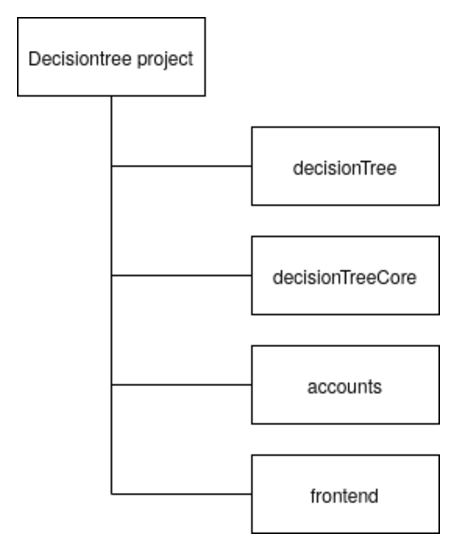
\includegraphics[height=8cm]{grafika/packages.eps}
	\caption{Podział projektu na moduły, źródło: opracowanie własne}
	\label{rys4_packages}
\end{figure}
%\subsection{Generowanie postępu}
Użytkownik po uruchomieniu zadania będzie widział procent zaawansowania tego zadania, jak i średni czas, który pozostał do końca. Zostało to rozwiązane w aplikacji poprzez tabelę w bazie pośredniczącą w wymianie informacji o zaawansowaniu danego eksperymentu. Program uruchomiony w robotniku Celery wypisuje informacje na standardowe wyjście. Z tych informacji pobierany jest numer wykonanej iteracji oraz średni jej czas. Stosując połączenie za pośrednictwem tzn. PIPE, proces robotnika Celery może przeanalizować te informacje. W celu ograniczenia obciążenia co dziesiąta linia jest poddawana analizie. Na podstawie zawartych tam danych oraz ilości uruchomień algorytmu uzyskanej z pliku konfiguracyjnego można wyliczyć średni czas pozostały do końca obliczeń. Natomiast pasek postępu zostaje wyznaczony poprzez określenie numeru ostatniej iteracji i stwierdzeniu ile wykonań algorytmu jeszcze pozostało. 

%\subsection{Autoryzacja użytkownika}
Autoryzacja użytkowników jest nieodłącznym elementem aplikacji internetowej. W tym celu został wykorzystany mechanizm tokenów. Taki token zostaje przyznawany użytkownikowi po zalogowaniu lub samej rejestracji. Umożliwia on autoryzowany dostęp do strony internetowej i dołącza się go w każdym zapytaniu. Po stronie wizualnej aplikacji jest przechowywany w \textit{local storage} przeglądarki internetowej. Każdy token posiada swój czas aktywności, a po jego wygaśnięciu lub przy dowolnym problemie z jego uwierzytelnieniem użytkownik zostanie przekierowany na stronę główną. 

\section{Przechowywanie danych}
W celu przechowywania danych została wykorzystana relacyjna baza danych PostgresSQL. Całość działa  na oddzielnym kontenerze w celu uzyskania większej stabilności i nie zależności od głównego modułu aplikacji. Schemat struktury wszystkich tabel przedstawiono na Rys. \ref{rys5_database_schema}. Większość tabel wynika z samego zastosowania frameworka Django i DjangoRestFramework. Wykorzystując gotowe moduły zostały zapewnione takie modele encji jak \enquote{auth\_user} odpowiadający za zapisywanie informacji o użytkownikach, czy też \enquote{authtoken\_token} mający na celu przetrzymywanie tokenów autoryzacji. Do całej struktury zostały dodane dodatkowe tabele:
\begin{itemize}
	\item \enquote{decisionTreeCore\_experiment} przetrzymująca dane o eksperymentach,  
	\item \enquote{decisionTreeCore\_permissions} zawierająca informacje o prawach dostępowych do eksperymentu,
	\item \enquote{decisionTreeCore\_progress} składa się z pól określających postęp wykonywania doświadczenia.
\end{itemize}



\begin{figure}[htb]
	\centering
	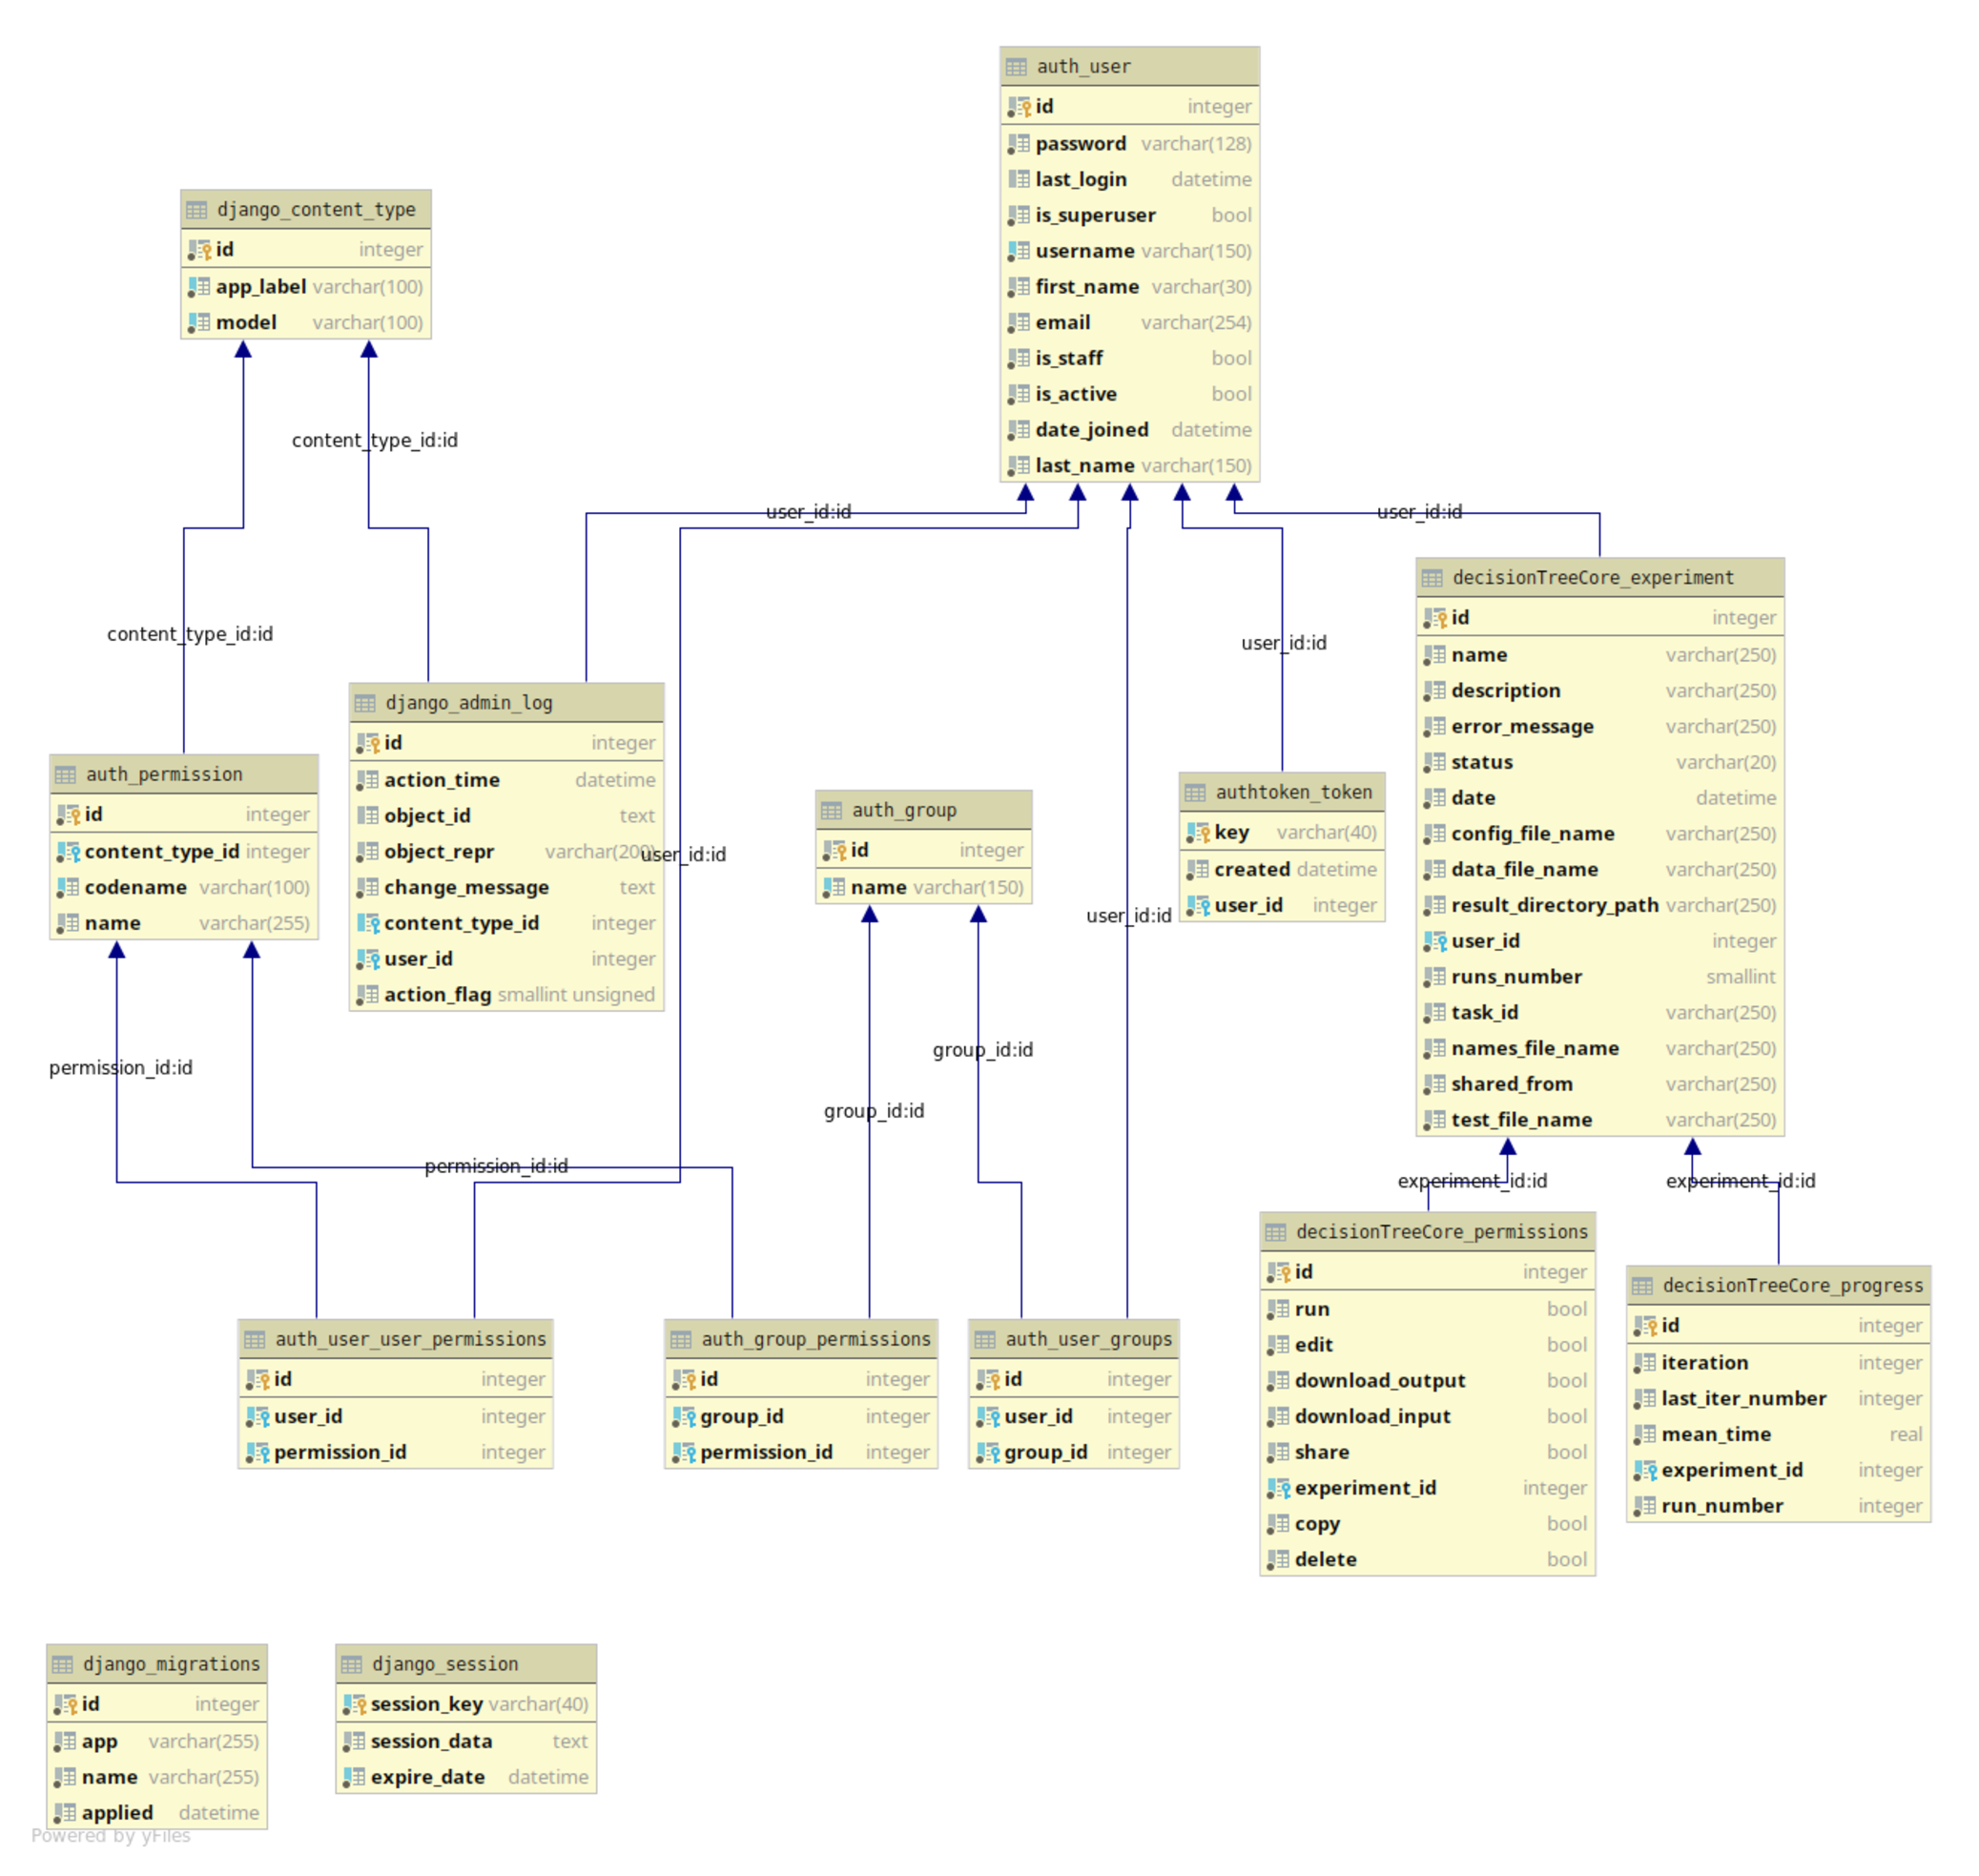
\includegraphics[angle=270, width=16cm]{grafika/database_schema.eps}
	\caption{Schemat bazy danych, źródło: opracowanie własne}
	\label{rys5_database_schema}
\end{figure}

 
\begin{figure}[htb]
	\centering
	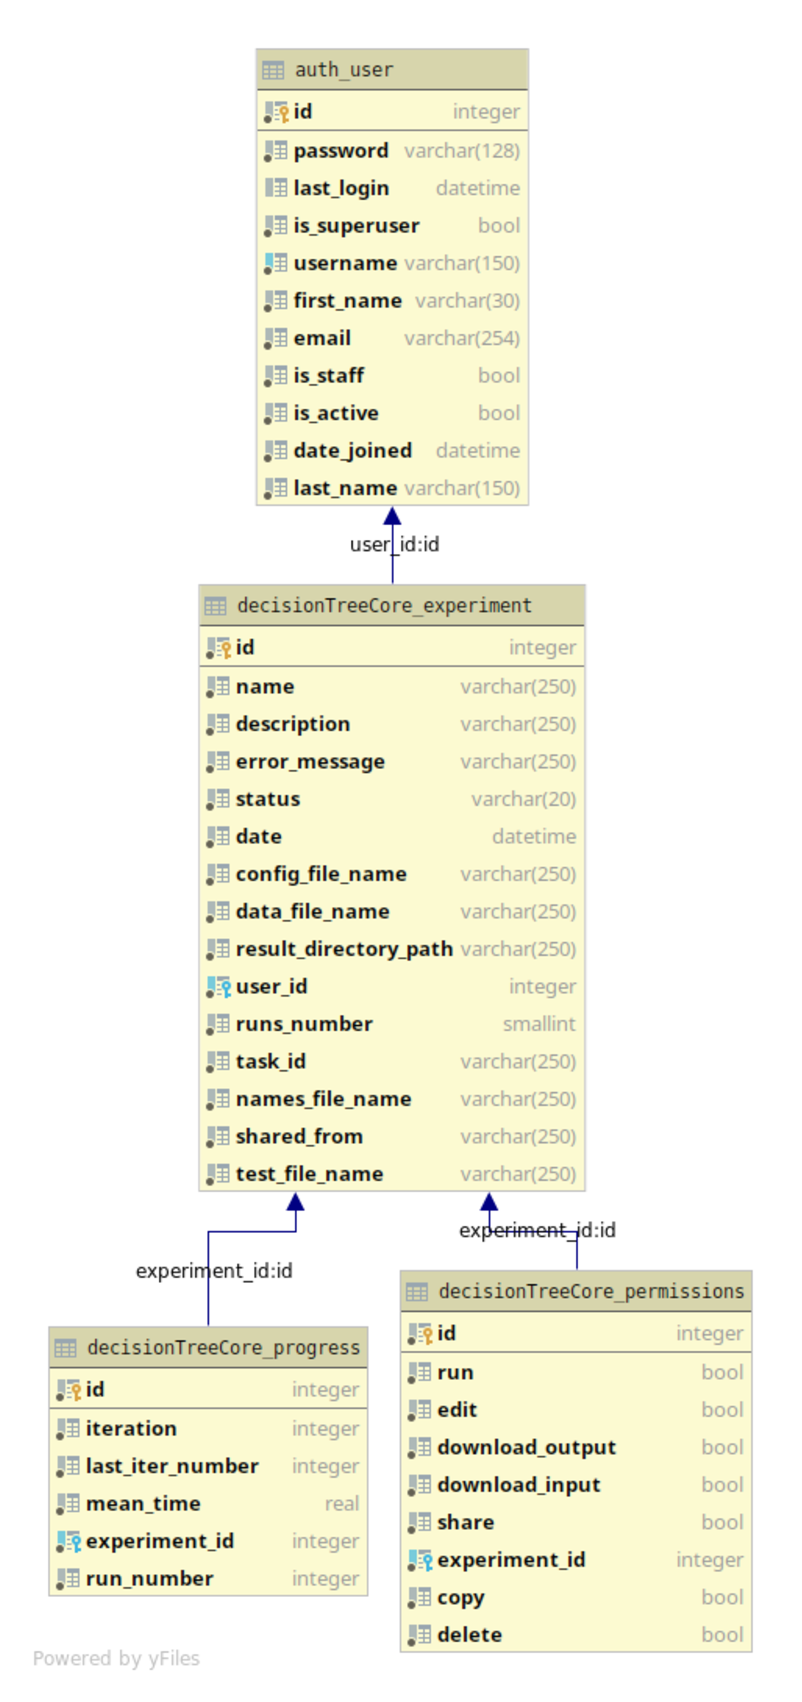
\includegraphics[height=16cm]{grafika/database_schema_2.eps}
	\caption{Schemat tabel dodatkowych, źródło: opracowanie własne}
	\label{rys6_database_schema}
\end{figure}

\begin{table}[htb]
	\caption[Opis pól tabeli \enquote{decisionTreeCore\_experiment}]{ Opis pól encji \enquote{decisionTreeCore\_experiment}}
	\centering
	\begin{tabular}{|c|c|p{9cm}|}
		\hline
		\textbf{Nazwa pola} & \textbf{Typ} & \textbf{Opis} \\\hline
		id & integer & Klucz główny tabeli \\\hline
		name & varchar(50) & Nazwa eksperymentu\\\hline
		description & varchar(250) & Opis eksperymentu\\\hline
		error\_message & varchar(250) & Wiadomość o błędzie, który wystąpił podczas uruchomienia eksperyment\\\hline
		status & varchar(15) & Pole określające w jakim statusie znajduje się eksperyment. Możliwe wartości to: \enquote{Created}, \enquote{In queue}, \enquote{Running}, \enquote{Finished}, \enquote{Error}. Zmiana statusów następuje w trakcie przechodzenia eksperymentu przez kolejne etapy\\\hline
		data & datetime & Data stworzenia eksperymentu przez użytkownika\\\hline
		config\_file\_name & varchar(50) & Nazwa pliku konfiguracyjnego użytego w eksperymencie\\\hline
		data\_file\_name & varchar(50) & Nazwa pliku zawierającego zbiór uczący \\\hline
		test\_file\_name & varchar(50) & Nazwa pliku zawierającego zbiór testowy \\\hline
		names\_file\_name & varchar(50) & Nazwa pliku określającego nazwy klas oraz rodzaj zmiennych \\\hline
		result\_directory\_path & varchar(50) & Ścieżka do folderu z wynikami eksperymentu\\\hline
		user\_id & integer & ID użytkownika, który jest właścicielem eksperymentu \\\hline
		runs\_number & smallint & Pole określające ile przebiegów algorytmu ma się odbyć podczas uruchomienia eksperymentu w systemie GDT. Pełni ważną rolę przy tworzeniu paska postępu oraz określeniu liczby wyświetlanych drzew\\\hline
		task\_id & varchar(250) & Zawiera id zadania, które trafiło do robotnika Celery. Umożliwia zarządzanie danym zadaniem np. usunięcie z kolejki, lub anulowanie w trakcie trwania\\\hline
		shared\_from & varchar(250) & Pole pełni rolę zapisu informacji o poprzednich właścicielach. W wartością pola są nazwy użytkowników. Podczas kolejnych udostępnień do pola są dodawane po przecinku następne loginy  \\\hline
	\end{tabular}
	\label{tabela_1_schema_experiment}
\end{table}

\begin{table}[htb]
	\caption[Opis pól tabeli \enquote{decisionTreeCore\_progress}]{ Opis pól encji \enquote{decisionTreeCore\_progress}}
	\centering
	\begin{tabular}{|c|c|p{9cm}|}
		\hline
		\textbf{Nazwa pola} & \textbf{Typ} & \textbf{Opis} \\\hline
		id & integer & Klucz główny tabeli \\\hline
		iteration & integer & Liczba iteracji eksperymentu\\\hline
		last\_iter\_number & integer & Numer ostatniej iteracji\\\hline
		mean\_time & real & Wiadomość o błędzie, który wystąpił podczas uruchomienia eksperyment\\\hline
		experiment\_id & integer & Numer id eksperymentu, do którego jest przypisany postęp \\\hline
		run\_number & integer & Numer określający, które uruchomienie algorytmu właśnie trwa\\\hline
		
	\end{tabular}
	\label{tabela_2_schema_progress}
\end{table}

\begin{table}[htb]
	\caption[Opis pól tabeli \enquote{decisionTreeCore\_experiment}]{ Opis pól encji \enquote{decisionTreeCore\_permissions}}
	\centering
	\begin{tabular}{|c|c|p{9cm}|}
		\hline
		\textbf{Nazwa pola} & \textbf{Typ} & \textbf{Opis} \\\hline
		id & integer & Klucz główny tabeli \\\hline
		run & bool & Prawo do uruchamiania eksperymentu\\\hline
		edit & bool & Prawo do edycji\\\hline
		download\_out & bool & Prawo dające możliwość pobierania plików wyjściowych\\\hline
		download\_in & bool & Prawo dające możliwość pobierania plików wejściowych\\\hline
		share & bool & Pozwolenie do dalszego udostępniania eksperymentu\\\hline
		copy & bool & Prawo do tworzenia kopii\\\hline
		delete & bool & Prawo do usunięcia eksperymentu\\\hline
		experiment\_id & integer & Numer id eksperymentu, do którego są przypisane prawa dostępowe\\\hline
		
	\end{tabular}
	\label{tabela_3_schema_permissions}
\end{table}


Relacja pomiędzy nowo stworzonymi tabelami, a użytkownikiem została przedstawiona na Rys. \ref{rys6_database_schema}. Tabela \enquote{decisionTreeCore\_experiment} zawiera informacje o pojedynczym eksperymencie użytkownika, w Tab. \ref{tabela_1_schema_experiment} znajduje się opis jej pól. W celu śledzenia postępu danego doświadczenia została stworzona tabela \enquote{decisionTreeCore\_progress}. Poszczególne pola zostały rozpisane w Tab. \ref{tabela_2_schema_progress}. Dane do tej tabeli są wpisywane prosto z robotnika Celery, przy czym brana jest pod uwagę tylko co dziesiąta iteracja systemu GDT. Zakres uprawnień do eksperymentu określa ostatnia tabela \enquote{decisionTreeCore\_permissions}. Schemat pól encji został rozpisany w Tab. \ref{tabela_3_schema_permissions}. Prawa dostępowe do doświadczenia są definiowane przez użytkownika przed samym udostępnieniem. Kolejny właściciel nie może rozszerzyć uprawnień uprzednio zablokowanych.  





\subsection{Mechanizm kontroli wersji eksperymentu}
Nierzadko zdarza się tak, że użytkownik będzie chciał powtórzyć zadanie z tymi samymi parametrami albo zechce je trochę zmienić. Innym przypadkiem wymagającym częstego ponownego uruchamiania eksperymentu może być zmiana plików z danymi wejściowymi. Oba ta przypadki wymagają ingerencji w plikach doświadczenia, co może powodować problem, z traceniem poprzednich wyników. Rozwiązaniem tej kwestii może być na przykład tworzeni kopi eksperymentu za każdym razem, gdy następuje zmiana danych. Niestety wiąże się to ze zwiększeniem rozmiaru listy eksperymentów. W związku z tym został zaimplementowany mechanizm przechowywania poprzednich wersji eksperymentu. Przy każdej zmianie dowolnego pliku wejściowego, stare pliki zostaną zachowane poprzez dodanie na początku nazwy \enquote{\_old}. W przypadku, gdy plik o takiej nazwie już istnieje na koniec nazwy jest dołączany kolejny numer porządkowy w nawiasach. Dzięki temu użytkownik w dowolnym momencie może pobrać archiwum z plikami i zobaczyć stare ustawienia.

Należało założyć, że jedno doświadczenie może być przeprowadzane kilka razy, co powoduje kolejny problem z~nadpisywaniem plików wyjściowych. W aplikacji zostało to rozwiązane poprzez dodanie do mechanizmu kontroli wersji eksperymentu, dodatkowych funkcjonalności. Z każdym ponownym uruchomieniem doświadczenia automatycznie robi się kopia zapasowa poprzedniego folderu wyjściowego. Do nazwy katalogu jest dodawany na końcu przedrostek \enquote{old\_}, w~przypadku gdy już taka nazwa istnieje w systemie plików zostaje dodany numer porządkowy w nawiasach. Tak samo jak w poprzednim przypadku użytkownik po pobraniu plików, może obejrzeć poprzednie pliki wyjściowe. 

Dodatkowym mechanizmem zaimplementowanym w aplikacji jest tworzenie pliku \enquote{readme.txt}. Zabezpiecza on przed straceniem informacji o eksperymencie w przypadku awarii bazy danych. Przechowuje on informacje takie jak nazwy plików wejściowych czy też nazwę eksperymentu. Na tej podstawie w dowolnej chwili istnieje możliwość odtworzenia struktury w bazie danych. Przykład zawartości takiego pliku jest widoczny w List. \ref{list1_readme}.

\begin{lstlisting}[numbers=none,frame=single, caption={Przykład zawartości pliku readme },captionpos=b, label=list1_readme]
Information about created experiment: 
Experiment id: 4669
Experiment name: testowy_eksperyment
Files used in experiment: 
- config: test.xml,
- data: chess3x3x10000.data, 
- test: chess3x3x10000.test, 
- names: chess3x3x10000(1).names
\end{lstlisting}


\section{Wdrożenie aplikacji}
Aplikacja została wdrożona na serwer posiadający 2 GB RAM, procesor o częstotliwości taktowania 2 GHz oraz dysk SSD. Spełnia on podstawowe wymagania pod względem sprzętowym, przy założeniu niedużego obciążenia aplikacji. Do uruchomienia projektu jest potrzebna zainstalowana instancja platformy Docker. Dzięki konteneryzacji proces wdrożenia projektu przebiega bardzo prosto i ogranicza się do pojedynczej komendy aplikacji docker-compose. Po uruchomieniu oprogramowanie działa w tle i świadczy usługi użytkownikom. Dostęp do aplikacji jest możliwy przez dowolną przeglądarkę internetową poprzez przejście pod adres \enquote{http://decisiontree.pl}. Przykładowymi danymi do logowania są: 
\begin{itemize}
	\item nazwa użytkownika: \enquote{test\_default},
	\item hasło: \enquote{test\_default}.
\end{itemize} 
